\documentclass[12pt]{extarticle}

\usepackage{geometry}
\usepackage{amsthm}
\usepackage{amssymb}
\usepackage{amsmath}
\usepackage{graphicx}
\usepackage{hyperref}
\usepackage{float}
\usepackage{mathrsfs}

\renewcommand{\baselinestretch}{1.5}
\graphicspath{ {./images/} }

\geometry{a4paper,
 left=25mm,
 top=25mm}

\title{Supervised Deep Learning for Optimized Trade Execution}
\author{Hua Wanying, Long Zijie, Wang Kunzhen}

\begin{document}
\maketitle

\section{Introduction}
Optimized Trade Execution is one of the best-studied problems in the field
of quantitative finance. In this problem, the goal is to buy(sell) a given
number, V, of a specific stock within the given time horizon, H, with the
minimum total cost(maximum total gain). If there is remaining inventory
approaching the end of the time horizon, the agent will be forced to place
a market order. \\


\noindent Note the equivalence of both sides (the buy and sell side) of the
problem, we will therefore solve the problem only for the sell side. That is,
the goal of our model would be to maximize the total selling cost of the
V shares of a stock given the time horizon H. Moreover, we also note that
the problem is additive with respect to different stocks. That is, a problem
to buy $V_1$ shares of Stock A and sell $V_2$ shares of Stock B within a given
time horizon H has a solution equivalent to the addition of optimal solutions given by
solving the problem for Stock A and Stock B individually.\\


\noindent Our contribution to the study of the problem is to provide an alternative
approach to addressing the problem, referencing the reinforcement learning model in
\cite{reinforcement}. The model we build is based on supervised deep learning.
Implementation details, results as well as relevant justifications for the choices
and assumptions made for building the model are also provided in this report.
\section{Literature Review}

Our study originates from \cite{reinforcement} - the first large-scale empirical application of reinforcement learning to Optimized Trade Execution. It applies \textbf{state-based strategies} that examine salient features of the current order books in order to decide what to do in the next period, then fuses \textbf{dynamic programming} and exploits the approximate independence between private and market variables to find the best possible strategy. These concepts are well understood and implemented similarly in our algorithm. We also noted that its model performance is evaluated by comparing with a submit \& leave strategy at mid-spread. Such metric can be misleading in adverse market conditions, where mid-spread order will not be executed. Additional metrics is used to evaluate our model performance.
\section{Model}
In this project, we assume that the optimal execution strategy can be expressed as
a pure function of the following 6 variables: $t$ the remaining time before the end of
the time horizon, $i$ the remaining inventory to sell, the price level, price trend,
limit order book volume mismatch as well as the bid-ask spread at the decision point.
Following the convention in \cite{reinforcement}, we group the 6 input variables
into two categories, i.e., the \textbf{private variables} consisting of $t$ and $i$
that is specific to the Optimized Trade Execution problem, and the \textbf{market variables}
consisting of the rest of the four. Output of the model is represented by \textit{\textbf{action}},
the price at which to place a limit order.
The model can be expressed mathematically as
$$ \textit{action} = f(t, i, \textit{price level}, \textit{price trend}, \textit{vol mismatch}, \textit{bid-ask spread}), $$
where $f$ is an unknown function to be learned. \\


\noindent To estimate the function $f$, we develop a supervised deep learning model (thereafter referred to as \textit{the model}) as described below.
The model is implemented with \textit{Tensorflow} and \textit{Tensorflow
Keras} provided by Google Brain, using \textit{Python}.
Implementation of the model can be found in the file \textit{Model.py}.
\begin{figure}[h]
\centering
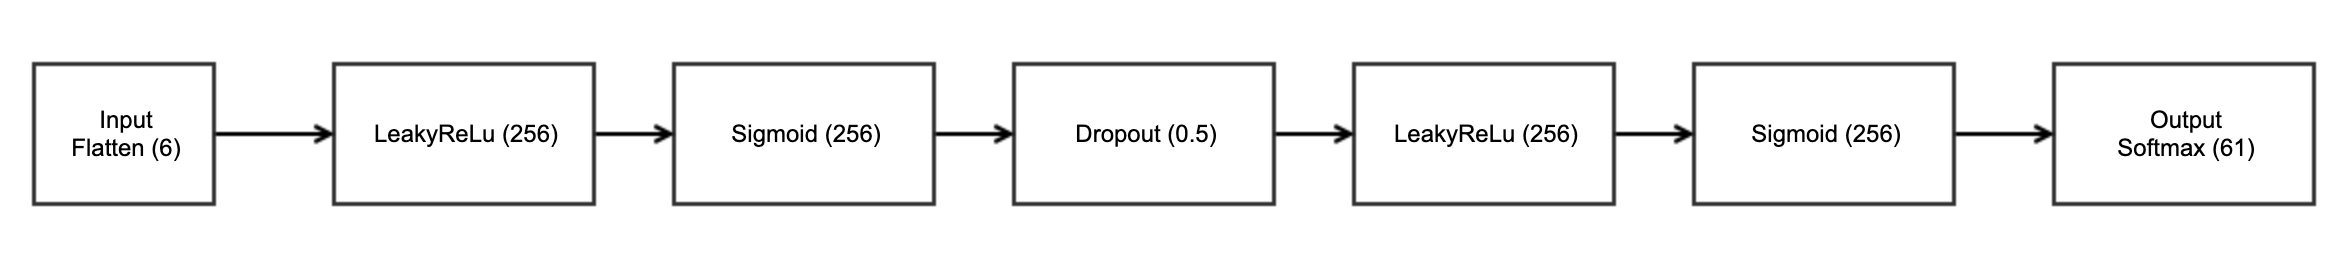
\includegraphics[width=0.7\textwidth]{model}
\caption{The Supervised Deep Learning Model}
\end{figure}

\begin{itemize}
\item \textbf{Input Layer} The input layer consists of simply the 6 parameters of the function $f$.
Detailed definitions, rationales and extractions of these variables are
provided in Section \ref{market-variables} and \ref{private-variables}.

\item \textbf{Hidden Layers} The model is composed of 5 fully-connected hidden layers with
256 neurons each. Activation functions for each layer is, correspondingly,
\textit{leakyReLu},
\textit{sigmoid}, \textit{dropout} with a rate of 0.5,
\textit{leakyReLu}, \textit{sigmoid}. These activations are
chosen after taking into consideration the nature of the
problems. For example, noting the sparse activation characteristic of
the \textit{leakyReLu} activation and that the outputs are discrete, we chose \textit{leakyReLu}
to denoise the training process. Another advantage of the \textit{leakyReLu}
is its computational efficiency and ability to avoid dead neurons.
The \textit{sigmoid} activation is chosen for its ability to capture
non-linear relationships. A \textit{Dropout} layer is chosen
in the middle to denoise and speed up the descent.

\item \textbf{Output Layer} The output layer represents the predicted action given
the input. The output variable, \textit{\textbf{action}}, is discrete for computational
efficiency. Moreover, having a discretized output is important to avoid overfitting.
Refer to Section \ref{private-variables} for details on how \textit{\textbf{action}}
is discretized.

\end{itemize}


\section{Data Preparation}
We choose the number of stock $V$ to be 1000 to ensure sufficient liquidity for market order given the order book data.
Time Horizon $H$ is set to be 120 seconds. Number of distinct points at which the policy is allowed to observe, $T$, is set to be 4, i.e. we can submit a revised limit order every $H/T$=30 seconds. Number of inventories units our policy can distinguish, $I$, is set to be 4, i.e. our order size is a multiple of $V/I$=250. These variables are chosen to simulate realistic task to sell stocks, to allow sufficient time for price fluctuations and also strike a balance for faster implementation.

\subsection{Data Description}
We use 3 month of high-frequency order book and message book data with stock Activision (ticker: ATVI). 2-month of data is used for model training and remaining 1 month for testing.
With order book data, we will be able to construct a 5-level sell order book and buy order book.
Message book data describes all historical events with time stamp, e.g. submission of a new limit order, deletion of a limit order and execution of a visible limit order. Please refer \href{https://lobsterdata.com/info/DataStructure.php}{\textbf{here}}
for details on data structure.

\subsection{Market Variables} \label{market-variables}

Firstly, we define some variables:
\begin{itemize}
  \item bid and ask price at the beginning of each interval : $bp_{beginning}$, $ap_{beginning}$
  \item bid and ask price at the decision point : $bp_{decision}$, $ap_{decision}$
  \item window length of moving average : $w$
  \item bid and ask order volume at decision point : $bv_{decision}$, $av_{decision}$
\end{itemize}
We calculate the market variables as following formulas:
\begin{itemize}
\item \textbf{Spread} : $ap_{beginning} - bp_{beginning}$
\item \textbf{Price level} : $\frac{\sum_{i=1}^{w}ap_i - ap_{decision}}{ap_{decision}}$
\item \textbf{Mismatch} : $bv_{decision} - av_{decision}$
\item \textbf{Trend} : $ap_{decision} - Price level$
\end{itemize}

Spread is the reflection of market liquidation, and order mismatch can measure the demand and supply in the market. These two market variables may tell us is the market a buyer's market or a seller's market. Meanwhile, if the price is at a high level, we prefer to sell orders as much as possible, vice versa. Although the price level of different period can be similar, we also need to consider the price momentum. For a seller, the upward trend is an opportunity.
\subsection{Private Variables} \label{private-variables}

\subsubsection{Trade Simulation}
We consider below different scenarios to simulate our order:
\begin{enumerate}
 \item $t = T$ (e.g. end of 120s) $\rightarrow$ market order $\rightarrow$ continue to sell at next available buy order until $i=0$
 \item $t = 0$ to $T-1$ $\rightarrow$ limit order
\end{enumerate}
 \begin{itemize}
 \item If order price $\leqslant$ best bid price $\rightarrow$ immediate execution $\rightarrow$ execution order of the same ID will not be executed again
 \item If best bid price $\leqslant$ order price $\leqslant$ best ask price $\rightarrow$ our limit sell order becomes the best ask price
 \item If order price $\geqslant$ best ask price $\rightarrow$ our order will not be executed even there is a buy order with price higher than our sell order
 \end{itemize}
\textbf{Note}: We have to always monitor all sell orders with higher priority to sell than ours, i.e. maintain a accurate sell order book. This includes tracking of sell order submission \& cancellation, sell book order execution.
\\Please refer \href{https://github.com/wangkunzhen/Machine-Learning-5225/blob/master/ExecutionEngine.py}{\textbf{here}} for trade simulation code.

\subsubsection{Dynamic Programming}

In this algorithm, we \textbf{iterate backwards in time}, solving first the state for $t = T$ and iterate the same procedure back to $t = 0$. Following graph visualize the process of dynamic programming.

\begin{figure}[H]
\center{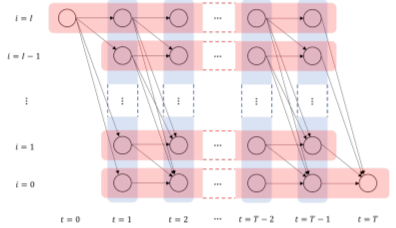
\includegraphics[width=0.7\textwidth]{visualization}}
\caption{Optimal path problem visualization}
\end{figure}

\noindent At $t = T$, the cost is knowable for any $action\in \mathscr{A}$, which is the optimal solution at time $T$.
$$c_T(i,\forall a \in \mathscr{A}) = market cost_{i,T}$$
At $t = T-1$ to $0$, we go through all possible action and inventory with knowing the inventory and maximum revenue at $t-1$,
$$c_{t-1}^{optimal}(y_{t-1},p_{t-1}) = Max\{c_{t}^{optimal}(y_t,p_t) + c_{t-1}(i,a) \quad for \quad a\in \mathscr{A}, i \in \mathscr{I}\}$$
where $y_t$ and $p_t$ is the remain inventory and action corresponding to the optimal strategy at time $t$.
\\Please refer \href{https://github.com/wangkunzhen/Machine-Learning-5225/blob/master/OptimizationEngine.py}{\textbf{here}} for dynamic programming code.




\section{Model Training}
For model training, we've experimented with quite a few model constructions, from which
we settled at the following configurations.\\


\noindent Firstly the loss function is determined to be the
\href{https://github.com/tensorflow/tensorflow/blob/r1.13/tensorflow/python/keras/backend.py}{\textbf{sparse categorical crossentropy}}
loss provided by \textit{Tensorflow Keras}. The loss function is one of the standard
choices in multi-categorization models, measuring the categorical crossentropy. \\


\noindent For optimization algorithm, we choose the widely used \textbf{Adam Optimizer} \cite{adam}.
It employes an adaptive learning rate and has a relatively efficient computational cost,
making use of both the first and second moments of the gradients. Key update routine
adopted by Adam is listed below.

\begin{equation*}
  \begin{split}
    g_t &\leftarrow \nabla_{\theta} f_t (\theta_{t-1}) \text{(Get gradients w.r.t. stochastic objective at time t)} \\
    m_t &\leftarrow \beta_1 \cdot m_{t-1} + (1-\beta_1) \cdot g_t \text{(Update biased first moment estimate)} \\
    v_t &\leftarrow \beta_2 \cdot v_{t-1} + (1-\beta_2) \cdot g_t^2 \text{(Update biased second moment estimate)} \\
    \hat{m_{t}} &\leftarrow \frac{m_t}{1 - \beta_1^t} \text{(Compute bias corrected first moment estimate)} \\
    \hat{v_{t}} &\leftarrow \frac{v_t}{1 - \beta_2^t} \text{(Compute bias corrected second moment estimate)} \\
    \theta_t &\leftarrow \theta_{t-1} - \alpha \cdot \frac{\hat{m_t}}{\sqrt{\hat{v_t}} + \epsilon} \text{(Update parameters)}
  \end{split}
\end{equation*}


\noindent The model is trained with the aforementioned configurations for 2000 iterations,
at which point we note that the cost remains relatively stable and the accuracy stops
improving. Therefore, we stop the training process at 2000 iterations.

\section{Results} \label{results}

We implement two cateogiries of metrics to evaluate the model, namely,
\begin{enumerate}
  \item \textbf{Accuracy}-based
  \item \textbf{Total Strategy Execution Cost}-based
\end{enumerate}
In this section, we define each of the two types of metrics and present their results correspondingly.

\subsection{Accuracy}
This is referred to as the accuracy metric, as defined by
$$\textit{accuracy} = \frac{\textit{count}(\textit{prediction} == \textit{label})}{\textit{count}(\textit{predictions})}.$$
Ultimately it measures how often the prediction matches the label provided, for both in-sample and out-of-sample data.
Fortunately we have a default implementation provided by
\href{https://github.com/tensorflow/tensorflow/blob/r1.13/tensorflow/python/ops/metrics_impl.py}{\textit{Tensorflow Keras}}. \\


\noindent We calculate the percentage in terms of decision points instead of training episodes. That is,
assume that we have $K$ training episodes in total with $D$ decision points each and
out of the $K \times D$ predictions we have $P$ predictions hitting the optimal decision,
the percentage calculated would be $\frac{P}{K \times D}$. On average, we are able to achieve
$54\%$ in-sample accuracy and $53\%$ out-of-sample accuracy.


\subsection{Total Strategy Execution Cost} \label{tsec}
\textbf{Total Strategy Execution Cost} is defined as the total cost if the client were to
completely follow the model's suggested actions at each decition point. Assume that
we are allowed to make decision every T time unit. That is, during the total time horizon
of the problem definition, we are only allowed to make decisions at $t \in \{ kT: 0 \le k \le \frac{H}{T} \}$.
Here for simplicity, we assume that $\frac{H}{T}$ is whole. Let $o_t$ represent the set
of market variables at time $H - t$, $c_{im}(t, i, o_t)$ and $n_{im}(t, i, o_t)$ represents the immediate execution cost and
immediate execution volume in time interval $[H-t, H-t+T)$ with remaining inventory $i$ and market variable $o_t$ at time $H - t$.
Then the \textbf{Total Strategy Execution Cost} is defined recursively as
$$c(V, H) = c_{im}(H, V, o_H) + c(V - n_{im}(H, V, o_H), H - T).$$

\noindent Reusing the \textit{ExecutionEngine.py} class, we can easily calculate
$c_{im}(t, i, o_t)$ and $n_{im}(t, i, o_t)$ given $t, i, o_t$, thus $c(V, H)$.\\


\noindent There are two evaluation metrics based on the \textbf{Total Strategy Execution Cost}:
percentage by which the model underperforms the optimal solution in terms of the cost and the
percentage by which the model outperforms the mid-spread submit and leave strategy.
Results for both metrics are presented below correspondingly.

\subsubsection{Model VS Optimal}
The optimal strategy is the strategy one can ever achive assuming all market information for the whole
time horizon H is known at the beginning. That is, the market becomes deterministic.
However, reality is that the market is stochastic, therefore the strategy one can
achieve would be at most as good as the optimal strategy.\\


\noindent Out-of-sample results comparing the model with the optimal strategy are shown in Figure \ref{optimal}.
Assuming the optimal cost is $c_{opt}$ and the model cost is $c_{m}$, then the y-axis
is expressed as $$opt\% = \frac{c_{m} - c_{opt}}{c_{opt}}.$$
Recall that the problem is for selling, therefore $c_{m} \le c_{opt}$ and hence $opt\% \le 0$.
On average, the model is able to achieve $\bar{opt\%} = -0.1179\%$ for out-of-sample data.
The number shows that on average, we are only $0.1179\%$ worse than the optimal strategy.

\begin{figure}[h]
\centering
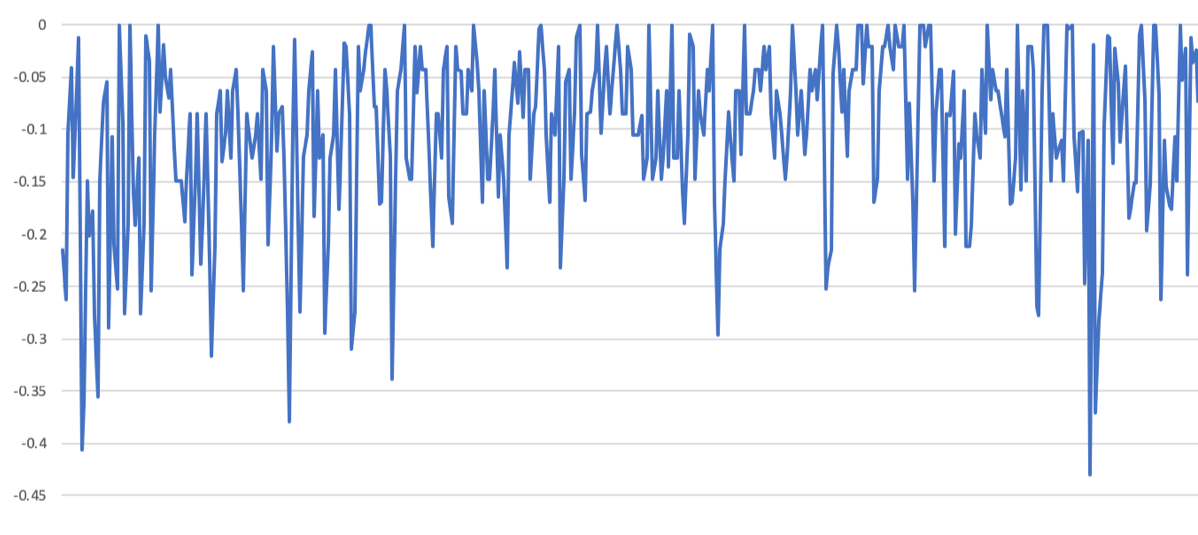
\includegraphics[width=0.7\textwidth]{optimal}
\caption{Percentage by which the model underperforms the optimal (\%)}
\label{optimal}
\end{figure}

\subsubsection{Model VS Mid-spread S\&L}

The mid-spread submit \& leave strategy is one that at the begining of the time
horizon H, we submit a limit order at the mid-spread price of the order book.
At the end of the time horizon H, all remaining inventory are submitted as market
order and assume to be executed at market price.\\


\noindent Out-of-sample results comparing the model to the Mid-spread submit \& leave strategy are shown
in Figure \ref{midspread}. Similar to the optimal case, assuming the mid-spread strategy
cost is $c_{mid}$, then the y-axis is $$mid\% = \frac{c_{m} - c_{mid}}{c_{mid}}.$$
On average, the model is able to achieve $mid\% = 0.54\%$.\\


\noindent Although this number seems small, it's actually quite significant, given that the
mid-spread submit \& leave strategy is on average only $0.7\%$ worse than the optimal.
Moreover, given our short time horizon H of 120 seconds and long decition interval
of 30 seconds each, we are only given 4 decision points for each training episode.
Therefore, if we were to follow the mid-spread price, it could be very hard to achieve the
goal of selling all the V shares within the horizon. Indeed, from Figure \ref{midspread}
we can observe two extreme points at which our model is significantly worse than
the mid-spread strategy. After tracing back the execution in the episode,
we realize that in those two periods if we were to follow the mid-spread strategy,
we wouldn't be able to sell all the V shares within H.


\begin{figure}[h]
\centering
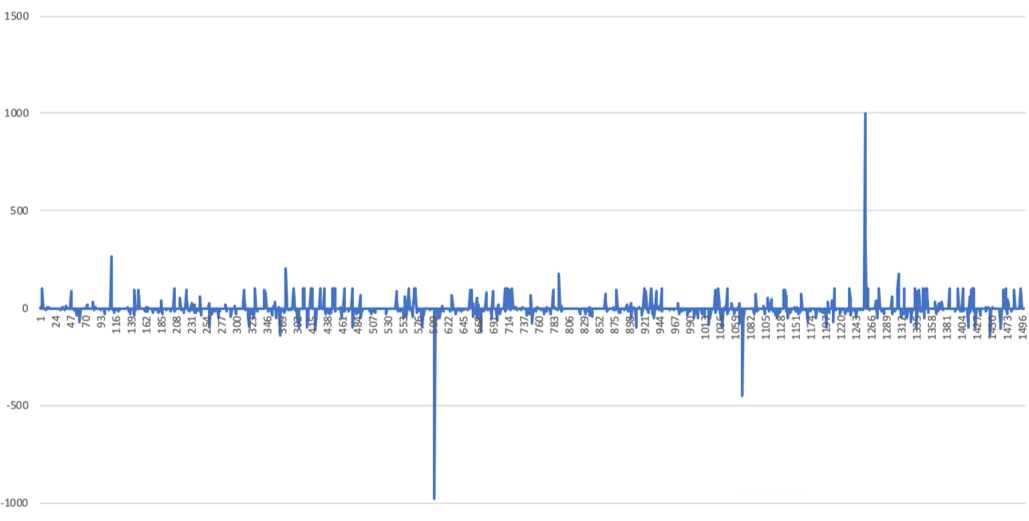
\includegraphics[width=0.7\textwidth]{midspread}
\caption{Percentage by which the model outperforms the mid-spread submit and leave (\%)}
\label{midspread}
\end{figure}

\section{Remarks \& Future Work}
Despite the satisfying performance of the model, there are still plenty of room
for future improvement. We have yet to implement the improvements due to time constraint
of the project. However, we would like to note them down here as remarks.

\begin{itemize}
  \item \textbf{Loss Function} For the current model training, the loss function is chosen as
  sparse categorical crossentropy to measure the categorical crossentropy.
  However, note that the label provided for the supervised training is the optimal
  strategy, having such categorical crossentropy losses might over-penalize the
  some of the predictions that could have done almost as good as the optimal solution
  in terms of total strategy execution cost, though having completely different decisions
  at each decision point. Therefore, a readily available alternative loss function
  would be the \textbf{total strategy execution cost} as defined in Section \ref{tsec}.\\


  We have implemented the loss function as per described in Section \ref{tsec}, but have yet
  to integrate it to the training process because the implementation requires
  extra inputs than those provided in the function signature required by \textit{Tensorflow Keras}.
  To actually integrate the loss function, further understanding of the \textit{Tensorflow Keras}
  framework is required.

  \item \textbf{Model Inputs} Current choices of the model inputs, especially the
  market variables, are somewhat arbitrary. We believe that further analysis is necessary
  to justify that the market variables chosen are sufficient to predict the actions.
  For example, a principle component analysis (PCA) should be performed for selection of the
  market variables.

  \item \textbf{Market Impact} Throughout our research, we have been assuming that
  there is no market impact for the limit order we placed. That is, we placing a new
  limit order to the market will not change the subsequent order book status except
  for an extra message book entry. However, this is definitely not true, especially
  when the volume becomes significant compared to the market volume. A model with such
  market impact factored in \cite{market-impact} must be employed for real-life application.
\end{itemize}

\section{Conclusion}
In this project, inspired by \cite{reinforcement}, we develop a supervised deep learning model for the optimized trade
execution problem. Sophisticated market simulation and dynamic programming algorithms
are implemented for prepartion of the model input to make it computationally more
efficient. Construction and training of the neural network is also fine-tuned with
efficiency and accuracy in mind. With \textit{Tensorflow} and \textit{Tensorflow Keras},
we are able to build and train the model with limited effort, and indeed the results of the
model are shown to be encouraging. Last but not least, we conclude the project with
a few important remarks and after-thoughts. It has been a fruitful journey.

\newpage
\begin{thebibliography}{9}
\bibitem{reinforcement}
Yuriy Nevmyvaka, Yi Feng, Michael Kearns.
\textit{Reinforcement Learning for Optimized Trade Execution}.
Proceedings of the 23rd International Conference on Machine Learning, Pittsburgh, PA, 2006.

\bibitem{adam}
Diederik P.Kingma, Jimmy Lei Ba.
\textit{Adam: A Method for Stochastic Optimization}.
ICLR, 2015.

\bibitem{market-impact}
Robert Kissel, Morton Glantz.
\textit{Optimal Trading Strategies: Quantitative Approaches for Managing Market Impact and Trading Risk}.
AMACOM, 2003.

\bibitem{literature-1}
Almgren, R., Chriss, N..
\textit{Optimal Execution of Portfolio Transactions}.
Journal of Risk, 2002.

\bibitem{literature-2}
Bertsimas, D., A, Lo, A..
\textit{Optimal Control of Execution Costs}.
Journal of Financial Markets 1, 1-50, 1998.
\end{thebibliography}

\end{document}
